\documentclass{article}
\usepackage[utf8]{inputenc}
\usepackage[english]{babel}
\usepackage{csquotes}

\usepackage{graphicx}               % image packages
\graphicspath{ {images/} }
\usepackage{float}
\usepackage{wrapfig}
\usepackage[rightcaption]{sidecap}

\usepackage[
backend=biber,
style=alphabetic,
citestyle=authoryear-comp 
]{biblatex}
 
\addbibresource{cs4099_bib.bib}     %imports bib file

\usepackage{hyperref}
\hypersetup{
    colorlinks,
    citecolor=black,
    filecolor=black,
    linkcolor=black,
    urlcolor=black
}

\title{CS4099: An Analysis of the Mechanisms and Techniques used in web-based Targeted Advertising}
\author{12001995}
\date{Academic Year 2015-2016}

\begin{document}

\maketitle

\begin{figure}[H]
  \centering
    
\includegraphics[width=0.8\textwidth]{university_logo.png}
\end{figure}

\pagebreak

\tableofcontents

\pagebreak

\section{Abstract}
The innovation of the world wide web has spawned  completely new forms of marketing and advertising. The most prevalent and insidious of these  is targeted advertising. The contemporary network of entities that interact to profile and track individuals and  bid for and place adverts within a website in real time is complex and lacks transparency. This project will  delve into the mechanisms and techniques used by organisations to i) profile individuals; ii) identify them when they are web browsing; iii) create and display targeted adverts to users in real time. It will also i) evaluate methodologies and tools designed to reduce the effectiveness of such advertising; ii) independently validate the background traffic associated with tracking; iii) create a framework of tools and methods to help improve the transparency of web tracking and profiling to the end user; iv) investigate the possibility for detecting digital advertising fraud through an app or plug-in.  

\section{Introduction}
There are numerous techniques used by advertising organisations to gain personal information of users for the purpose of targeted advertising, this paper will look to explore the various techniques and discuss how a user can increase their online privacy. The proceeding sections will present a number of the ways advertisers collect user data and how they are used.  

\subsection{Online Advertising}
Whilst it may seem like a relatively new concept, online advertising has been around since the beginning of the world wide web. The first clickable advert, which was later defined as a banner ad, was sold on the web by Global Network Navigator in 1993 to Heller, Ehrman, White, \& McAuliffe a law practice in Silicon Valley \parencite{oreilly}. The first mass production of advertising was implemented by \textit{HotWired.com} (now called Wired) which sold a large number of banner ads to corporate advertisers \parencite{firstAd}. These organisations where the at the cutting edge of advertising which then spawned into the complex ecosystem that online advertising is today.

\section{Targeted Advertising}
Online advertising is an increasingly broad category which takes up a large percentage of advertising budgets worldwide the forecasts of Satistia (2013) state that digital advertising increased to about 121 billion dollars in 2013 and is expected to double by 2018. The Federal Trade Commission (FTC) defines targeted advertising as ``the practice of tracking an individual’s online activities in order to deliver advertising tailored to the individual’s interests'' \parencite{comission2009}. Previous studies have stressed the privacy concerns about targeted adverting (Yang, et al., 2015) and analysed the effectiveness of targeted advertising (Brahim, et al., 2011) but this paper will focus upon the techniques used by targeted advertisers to create tailored online behavioural advertising. \newline

\subsection{Parties involved in Targeted Advertising}
One of the parties involved in targeted advertising is the Advertiser, this party will usually have a product that they wish to promote and are willing to pay for this promotion on a website e.g. \textit{Coca-Cola}. The publisher in this case is any website that is willing to give up real-estate on their page for an Advertiser's product e.g. \textit{gaurdian.com}. These two parties are normally connected by an Ad-network discussed in detail in Section \ref{AdNetwork} which has a large amount of advertising infrastructure and for a fee will facilitate it's services e.g. \textit{Google AdSense}. The parties can also be connected by an Ad Exchange discussed in Section \ref{AdExchanges}. Parties wishing to advertise can also utilise Demand Side Platforms to purchase digital advertising inventory this is discussed in Section \ref{DSP}. In contrast to DSPs, Supply Side Platforms can be utilised by web publishers to manage their advertising space inventory, filling it with adverts and receiving the corresponding revenue. This platform will be discussed in Section \ref{SSP}.  

% TODO: Research this
\subsection{Behavioural Re-targeting}
Adverts are a fundamental part of the web ecosystem. Users have begun to expect adverts for the latest line of sports trainers, whilst they are browsing the web site of an online clothes retailer. However, whilst surfing the Internet users are becoming increasingly aware of ``behavioural re-targeting'' where an advert which may have been viewed on a related page seemingly ``follows'' that user as they visit other unrelated web pages. This process is becoming increasingly prevalent as shown by a study of cookies in the top 100 web sites, in which an average of 57 cookies per web page was recorded \parencite{taOffer}. Whilst 20\% of pages visited contained 100 or more cookies \parencite{taOffer}. However, the most concerning fact about this discovery was that 87\% of cookies on these web sites were set by third-parties \parencite{taOffer}, this is where the re-targeting process begins as whenever the user visits a page within the same Ad Network (discussed in detail in Section \ref{AdNetwork}) the previous advert can be displayed to the user. \newline

\subsection{Ad Networks} \label{AdNetwork}
Online Ad networks began to appear in 1997. The original ad networks were created to address the problem of advertisers wanting to buy online inventory \parencite{adExchanges}. Internet audiences are incredibly fragmented, splitting their online time between many different websites. This is contrast to the traditional forms of media such as print, radio and television. By aggregating inventory across multiple sites, ad networks could offer advertisers the ability to reach the size of audience that they had come to expect from traditional channels of advertising. \newline

Ad networks can be defined as a company that connects advertisers to web sites that want to host advertisements. The key function of these networks is aggregation of ad space supply from publishers and matching it with advertiser demand. 

\subsection{Ad Server}
An Ad server is defined as the technology and services that places an advertisement upon a website. This technology can also be used to count the adverts, select more profitable locations for adverts and monitor the progress of different advertising campaigns. Ad Servers can be defined into two types: Publisher ad servers and advertiser or third party ad servers. \newline 

Typically an Ad server is a physical computer web server backed by a database server which can be used to store the advertisements and delivers them to website visitors. The contents of the web server is constantly updated so that the website which is used to display the ads contains fresh advertisements. The aim of ad serving is to deliver the content of adverts to users, to manage a websites advertising space and in the case of advertiser ad servers to provide an independent counting and tracking system to advertisers. \newline 

When Ad servers are run locally by a single publisher they can be used to serve ads to that publisher's domain, allowing fine-grained creative, formatting and content control by that publisher. Whereas remote ad servers can serve ads across domains owned by multiple publishers. This one centralised repository of adverts can allow advertisers and publishers to track the distribution of their online advertisements. 
\newline

\subsection{Demand Side Platform} \label{DSP}
The Demand Side Platform (DSP) can be described as software used to purchase advertising in an automated fashion. DSP facilitates a buyer with direct Real Time Bidding (RTB) access across multiple sources of inventory \parencite{introDSP}. Advertisers use DSPs to purchase impressions (an advertising slot) across a range of publisher sites, but targeted to specific users based on information such as their location and previous browsing history. Thus, enabling buyers to access a wider range of publishers and select the most appropriate for their requirements. For example Apple might recognise that a user has previously been on their site looking at a specific computer and therefore they may be prepared to pay more than Amazon or EasyJet to serve ads to the user. This process removed the human element of digital advertising which in turn improved the efficiency of the process whilst reducing the costs via automation. Publishers will make their impressions available through marketplaces called ad exchanges and then DSPs will automatically decide which impressions suit the requirements of the advertiser and purchase these impressions. Demand Side Platforms are offered by a large number of companies for example: App Nexus, Google DoubleClick, AdForm. 

\subsection{Supply Side Platform} \label{SSP}
A Supply Side Platform (SSP) is the publisher's equivalent of a DSP. Where DSPs are utilised by advertisers to buy ad impressions from exchanges in the most cost effective and efficient manner possible, SSPs are designed by publishers to do the opposite: to maximise the price an impression sells at. SSPs allow publishers to connect their inventory to multiple Ad Exchanges, DSPs and Ad networks at once. This increases the range of potential buyers dramatically which in turn can force the price of impressions higher and ensure that publishers get the highest possible rates therefore maximising the revenues they receive for their inventory. Whenever a Supply Side Platform is used to place an impression into various ad exchanges, DSPs will analyse and purchase them on behalf of marketers depending on attributes such as where they are served on the screen and which specific users they're being served to \parencite{introDSP}. Example of SSPs are: AppNexus Publisher Suite, Yahoo and OpenX SSP.  

\subsection{Real Time Bidding}
Real Time Bidding (RTB) is a deterministic process by which advertising inventory is bought and sold on a per-impression basis, via programmatic instantaneous auction, this approach is analogous to the financial markets \parencite{RTB}. With RTB advertising buyers bid on an impression in a real-time auction that occurs in the time it takes a web page to load. If the bid is won, the buyer's ad is instantly displayed on the publisher's site. These auctions are often facilitated by Ad Exchanges or Supply Side Platforms. One of the main advantages of Real Time Bidding is that is facilitates advertisers to manage and optimise adverts from multiple ad-networks by granting the user access to a multitude of different networks. Furthermore it gives advertisers the ability to create advertising campaigns on an instantaneous basis and allocate a much higher percentage of their unsold advertising inventory. \newline

In its simplest form, the RTB process unfolds much like the following: 
\begin{enumerate}
\item The publisher provides its inventory to an Ad Exchange, who is responsible for holding an auction, during which the DSPs, on behalf of the advertisers, will place a bid on each impression \parencite{howRTBWorks}. 
\item The value of the bid is based on the expected value of that impression to the advertiser based upon the parameters they have passed to the DSP. The auction process ensures that each impression is sold at as high a price as possible as dictated by the demand in the real-time market \parencite{howRTBWorks}. 
\item Once the bidding is over, the winner is chosen and their ad is served on the publisher's website. 
\end{enumerate}

\subsection{Data Management Platform}
To acquire the large amounts of data needed to target and potentially re-target users with advertisements many organisations have began to use Data Management Platforms (DMP). DMPs are essentially a data warehouse, a piece of software that is utilised to store, sort and report on the vast amount of data used by all businesses involved with the programmatic advertising process. In a similar manner to a database DMPs can be used to house and manage any form of information but marketers most often utilise the platform to manage cookie IDs and to generate audience segments, which are subsequently used to target specific users with online adverts \parencite{DMP}. As previously discussed the myriad of middlemen including DSPs, ad networks and exchanges makes it hard for advertisers to keep track of their performance. Therefore, a Data Management Platform can be used as one centralised repository to keep all audience data and resulting performance of advertising together, which allows advertisers to optimise future inventory purchasing and ad creativity. Examples of Data Management Platforms include: Oracle DMP (powered by BlueKai), Adobe Auidence Manager and Krux. \newline

DMPs can be used on both sides of the advertising ecosystem. Information can be fed from a marketer's DMP to its DSP to help inform ad purchasing decisions, but without being linked to another technology, a DMP is largely redundant. In contrast, DMPs can be 
utilised by publishers by linking them to a SSP. In this case, the DMP holds publisher information on its readers, which may help them to sell their adverts for a higher price. Like many of the areas discussed in this paper the line between DMPs and DSPs are largely artificial and are beginning to blur, as growing number of DSP providers now offer their clients DMP services too.  

\subsection{Ad Exchanges} \label{AdExchanges}
Ad Exchanges can be seen as the medium through which Ad impressions from publishers can be made available to potential buyers. An advert exchange is a technology platform that facilitates the buying and selling of media advertising inventory whose prices are determined through an online auction with bidding coming from multiple ad networks, this process is also referred to as Real Time Bidding. This approach is technology-driven as opposed to the traditional process of negotiating prices on media inventory. Examples of these platforms are: DoubleClick, AdECN, Rubicon Project and Open X. \newline

Whenever a user visits a website, in the short interval of the page load time, in the background an ad exchange conducts an auction between multiple advertisers for each impression on that page. The advertisers bid for the impression of the user and compare this to their target behavioural and demographic along with the subject matter of the website and the dimensions of the ad (including placement on the site). The highest bidder during the auction will win the right to place an ad on the website. This whole procedure takes place in ``real-time'' in the short number of milliseconds it takes for a web page to load, an example of the auction process is shown in Figure \ref{fig:adExchange}. 

\begin{figure}[H]
    \centering
    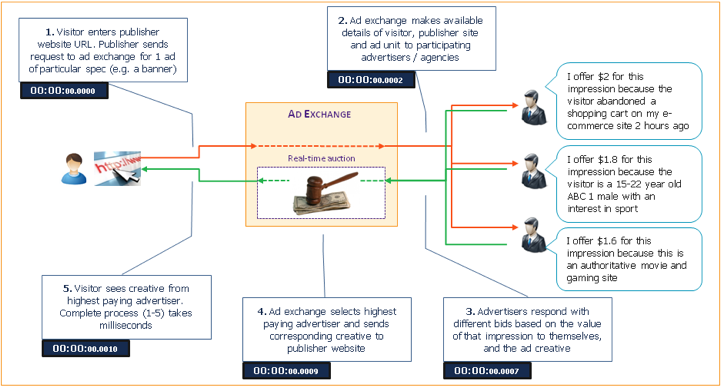
\includegraphics[width=1\textwidth]{adExchange}
    \caption{An example interaction on an Ad Exchange platform \parencite{adExchanges}}
    \label{fig:adExchange}
\end{figure}

\subsection{Targeted Ad Networks}
Targeted Ad networks differ from an Ad network by allowing advertisers to buy audience segments such as: demographics (e.g. gender, age),  behavioural segments (e.g. interest in buying a home), by context (e.g. websites that are in a particular subject area) or by alternatives to Cost Per Mile (CPM) such as cost per 1000 viewers of the advertisement. This holds a significant advantage to advertisers as it offers them the ability to buy on a performance basis. Similarly, this structure offers benefits to publishers who have the ability to sell remnant inventory without cannibalizing higher priced inventory sold directly via ad networks \parencite{adExchanges}. Examples of Targeted advertising networks include: Google AdSense, Yahoo! Publisher network and AOL Advertising. 

\subsection{Online Advertising Fraud}
One of the largest challenges in the paradigm of online advertising is how to ensure human users are actually seeing and then clicking through adverts. Bloomberg reported that 11\% of display ads and 25\% of video ads placed on the Internet in 2014 were seen by bots, instead of human users \parencite{bloomFraud}. This correlates with the research of the Financial Times newspaper that found that part of a Mercedes-Benz on-line advertising campaign was viewed more often by computer bots than by real human users. With legitimate human users amassing only 43\% of the views \parencite{mercFraud}. Advertising is suffering heavily from the prevelence of Bot Nets, which can be defined as a network of private computers infected with malicious software (malware)  and controlled as a group without the owners' knowledge. In the case of advertising fraud, bot nets are being used when publishers purchase traffic (views) for their website to help boost the price of their advertising inventory. Now that the purchasing of `fake traffic' is so ubiquitous in the advertising industry it has given rise to an industry of countermeasures \parencite{bloomFraud} where publishers are constantly battling the ever increasing number of fake or software related views. This will damage advertisers most, as they are forced to check whether their ads are being viewed by the ever increasing army of bots instead of potential human clients. A study conducted by the security firm White Ops for the Association of National Advertisers (ANA) concluded that adverts viewed by non-human traffic will cost advertisers \$6.3 billion in 2015. This shows the prevalence and scale of advertising fraud and that advertisers and publishers must work together to help to mitigate the effects of the fake traffic associated with bot nets. Publishers are currently using multiple methods to detect nonhuman traffic however, there is no single standard used by the industry. This form of fraudulent activity is the biggest threat to the online advertising industry. However, as long as publishers continue to by traffic to their website for the purpose of boosting their advertising revenues, this fraudulent activity looks set to continue. 


\subsection{Tracking}
In terms of this study, tracking will be defined as collecting the personal information and online movements of Internet users for the purpose of using this information to tailor adverts to these users. The most popular method used to collect this data is cookies which are discussed in Section \ref{cookies}. Increasingly advertisers are able to track a user's browsing activities across multiple websites, they can then collate all of this information and use it to better tailor their personalised adverts to an individual user. 

The merits of tracking has been the topic of much debate, as increasingly users feel that their privacy is under threat from intrusive advertisers who collect data using numerous methods. 

\subsection{Tracking Taxonomy}
One of the simplest ways to to classify tracking is based on the domain. There are two different domains for tracking \textit{within site} and \textit{cross site}. Within site tracking is when a first party cookie is used to track a user on the the website that user is viewing. Whereas, cross site tracking refers to tracking the preferences and online movements of Internet users on websites using third-party cookies. A framework has also been suggested which classifies web tracking based on the observable behaviours. This framework is shown in Figure \ref{fig:TAframework}  \parencite{roesner}. 

\begin{figure}[H]
    \centering
    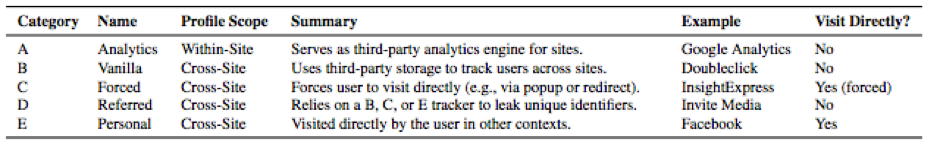
\includegraphics[width=1\textwidth]{TAframework}
    \caption{Framework for classifying web tracking based on observable behaviours \parencite{roesner}}
    \label{fig:TAframework}
\end{figure}

\section{The Arsenal of the Trackers}

\subsection {Cookies} \label{cookies}
A cookie can be defined as a triple (domain,key,value) that is stored in the browser across page visits, where the domain is a particular website and the key and value are opaque identifiers \parencite{roesner}. The cookie mechanism adds state to the otherwise stateless HTTP protocol, as the cookies allow a web server to store a small amount of data on the computers of the visiting users which is then sent back to the web server upon subsequent requests \parencite{cookielessMonster}. The information contained in the cookie could be about the user's previous browsing activity such as, logging in, clicking particular buttons and sites they have previously visited or it could contain stateful information for example what items they added to their shopping cart. Although the most controversial of cookies are those that are utilised to manage the advertising on a website, these cookies can be set from a separate advertising delivery company. This cookie can record when and where you saw an advert and whether you chose to click through the advert to purchase the product. This information will then be returned to the cookie owner who records the data and will use that to inform behavioural targeting for future adverts placed in front of a user.  \newline 

There are two types of cookies \textit{first-party} and \textit{third-party}. First-party cookies are set by the domain that the user visits directly, i.e. the domain in the address bar, for example, if a user visits www.google.com then cookies that are set with the domain of www.google.com are first party cookies. Third-party cookies are set by a different domain than the one the user visits, they are embedded in the top-level page, for example if a visitor visits www.amazon.com and the domain of the cookies added are www.google.com then these cookies are third-party cookies. \newline

There are numerous ways cookies can get to a webpage. Traditionally cookies were set by using an HTTP response that included a Set-cookie header, however cookies can appear in a browser in a numerous more subtle methods now. They can be set either by Javascript scripts running in the page or by using an API call from within a plug-in. Cookies are one of the simplest yet most effective ways to gain information about a user which can then be used for behavioural targeted advertising, or to build a profile about a user to place them in an audience segment. As the information in the cookie is constantly evolving dynamically with user actions it is very effective for trackers to place a cookie within a user's browser. 

% TODO: research this
\subsection{Supercookies} \label{Supercookies}
The term Supercookie is used to refer to methods used to uniquely identify users that do not rely on HTTP cookies. A supercookie generally refers to a means of storing something unique from a website on a user's computer so that it can be retrieved the next time the user visits that website. The name is rather misleading as these methods of tracking aren't technically cookies as they are not placed on a user's computer via the HTTP protocol. There are approximately 13 different supercookie storage methods, the most prevalent is ``Flash cookies". \newline 

The Local Shared Objects (LSOs) found within the Flash plugin are used to provide Flash applications with the ability to save options to the local system, for example, to save progress in a game. But as there is not a distinction between good and bad usage of this mechanism many websites have began to save persistent information on the user system as an alternative to third-party HTTP cookies. The output from this exploit is referred to as a ``Flash cookie" as a tracking organisation could use this method to place a uniquely identifiable data directly to a user's computer. Flash cookies are still a frequently used resource in the domain of tracking as a user cannot access them easily from within the browser. Flash cookies are not located with other HTTP cookies, easily accessible from a cookie manager in the browser, nor are they present in databases or other browser-specific storage locations \parencite{flashCookies}. A user must also travel to the Adobe Flash Player Settings Manager webpage (\url{http://www.macromedia.com/support/documentation/en/flashplayer/help/settings_manager07.html}) to manage or delete Flash cookies and update their related settings, which is both unintuitive and poorly documented. Therefore users who have cleared their HTTP cookies may think they are no longer being tracking, however websites utilising LSOs will still be able to track them. This process is not transparent to the user meaning that they can be unaware they are still being tracked. Another reason, why they are potentially favoured in a tracking context is that traditional HTTP cookies are limited in size to 4 Kilobytes of data whereas Flash cookies can be utilised to store up to 100 Kilobytes \parencite{flashCookies}. The larger storage capacity and difficulty in removing Flash cookies makes them an effective means of tracking even a privacy conscious user. Although the evolution of HTML5 has limited the appeal of Adobe's browser plugin Flash it still commands usage on 9.3\% of Internet sites whilst this is a far cry from 2010 where 28.5\% of global Internet sites used the plguin \parencite{flashStats}. Adobe reports that there are ``more than 500 million devices are addressable today with Flash technology, and it is projected there will be over 1 billion addressable devices by the end of 2015" \parencite{adobeFlash}. These statistics illustrate that although adoption rates of Flash may be slowing the Flash cookie method of tracking is still relevant and could be used to profile a huge number of users, most of which would be largely unaware they were being tracked. \newline 

% TODO: add more?
\subsection{Evercookies}
An evercookie is a resilient tracking mechanisms that uses multiple storage vectors including Flash cookies, localStorage, sessionStorage and ETags \parencite{evercookies}. Evercookies use this information to identify a client even after they've removed standard cookies. This is similar to the ``respawning" of cookies shown in \parencite{flashCookiesPrivacy} which illustrated the abuse of Flash cookies for regenerating previously removed HTTP cookies. The rationale behind evercookie API is to make stateful methods of tracking persistent. By storing the same data in a multitude of storage locations, if any tracking information is lost or removed it can simply be recovered from another storage location and then continue to be used for tracking purposes. At the time of writing this paper the evercookie API uses 13 different storage vectors to accomplish its persistence,  \parencite{evercookies}. Evercookies, are sometimes referred to as \textit{Zombie Cookies} due to the fact they are automatically re-created (respawned) from a backup outside the web browsers traditional cookie storage. Evercookies take advantage of a number of Supercookie techniques discussed in Section \ref{Supercookies} to restore the cookies. \newline

This abuse of the cookie platform is one of the biggest privacy concern for any Internet user, as these forms of stateful storage actively circumvent user's deliberate attempts to start with a fresh profile. As users have to be more than aware to remove all forms of tracking techniques, otherwise the methods previously can simply be respawned from any surviving storage. 

\subsection{Cookie Syncing}
Cookie synchronization or cookie syncing is the process of trakcer domains sharing pseudonymous IDs associated with a given user, typically stored in cookies \parencite{webNeverForgets}. This passing of IDs can occur for example when domain A makes a request to a URL hosted by domain B with the pseudonymous ID as parameter within the request. This can be advantageous for organisations as it provides a means for domains to share cookie values and thus the different domains should be able to utilise the information in the cookie to better target adverts to a user's preferences. Observed cookie syncing is indicative of business relationships.  One of the earliest studies of cookie syncing found over 100 syncing events happen on the top 100 Alexa sites \parencite{sellingPrivacy}. A slightly larger scale study was conducted by \parencite{webNeverForgets} and its results can be seen in Figure \ref{fig:cookieSynching}, which were generated from multiple crawls of the top 3,000 Alexa domains. 

\begin{figure}[H]
    \centering
    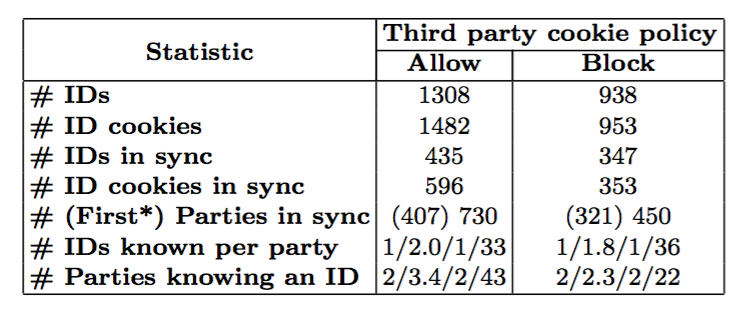
\includegraphics[width=0.75\textwidth]{cookieSynching}
    \caption{Cookie synching statistics from the study of \parencite{webNeverForgets}. The format of the bottom two rows is minimum/mean/median/maximum.}
    \label{fig:cookieSynching}
\end{figure}

These results show that cookie syncing is prevalent upon some of the most visited and trusted sites on the Internet, which would indicate it could ubiquitous across the Internet. The main incentive for trackers to share cookies is the ability to merge databases on the backend based upon the synced IDs. This form of sharing and merging allows trackers to aggregate data in order to obtain a larger fraction of a user's browsing history. As this backend merging occurs behind the closed doors of organisations there is a lack of transparency and information of how prevalent the technique is.  However, the financial and mutual benefits for organisations to share tracking information across the ecosystem are significant. As reported by \parencite{webNeverForgets}  101 domains could construct 50\% of a user's browsing history with third-party cookies enabled, this increase in ability to recreate a user's history could have large effects both on user privacy and targeted advertising effectiveness. \newline

The most concerning area of cookie syncing is that it is extremely difficult to block. There are not any tools specifically designed to combat cookie syncing, however a brute force approach would be to block third-party cookie placement and HTTP traffic \parencite{webNeverForgets}, although this lacks practicality. 

% Web Beacons aka Pixel Dropping
\subsection{Web Beacons}
A further technique used to track users in a transparent manner is the use of Web Beacons sometimes referred to as ``pixel dropping". The premise of this method is that when a user visits a webpage this site includes an object, which is used to unobtrusively and normally invisibly check whether the user has accessed the content. The common use case for this method of tracking is in web analytics and email tracking. For example, a web beacon can take the form of an invisible 1x1 pixel in which case it may be referred to as \textit{Pixel Tag}, although the form the beacon takes is largely irrelevant as the pixel can also be replaced with a script block, the beacon would then be referred to as \textit{Javascript tag}. This transparent GIF or PNG image can be embedded into an HTML page, whenever a user navigates to a page containing graphics the image is downloaded. This download requires the browser to a send a request to the server storing the image, allowing the organisation running that server to keep track of the HTML page \parencite{}. This therefore allows for third party sites to gather information about visitors when they pull HTML content from the main site. These sites can then in turn track (a section of) the browsing habits of a significant share of web users. Normally advertisements, banners and social media buttons are fetched from their origin site, not from the main site, therefore organisations such as Google, Facebook and Twitter can potentially view and utilise the browsing habits of a large proportion of Internet users and as these organisations' products are used ubiquitously across the Internet, their assets will appear on many websites meaning they can generate a much larger section of a user's browsing history.   Web beacons can be used in conjunction with HTTP to ensure that a cookie is downloaded and as most beacons are invisible to the user, the user may have unconsciously downloaded a wealth of third-party cookies simply from visiting one webpage. \newline

% invisible to user so privacy at risk
These beacons are usually invisible to users, therefore they present a serious privacy risk, as users could be completely unaware that they are being tracked. However, there is a defence to this the Ghostery browser extension analyses Javascript to detect trackers, pixels and beacons and can be used to block them. 
    
\subsection{Fingerprinting} \label{fingerprinting}
Another tool available to trackers is device fingerprinting, which aims to identify web users by tracking and collecting their information without the help of cookies. Benign characteristics of a browser's environment like the screen dimensions and list of installed fonts, could be combined to create a unique device-specific finger print, analogous to a human biological fingerprint \parencite{uniqueBrowser}. Fingerprinters use attributes that take more diverse values (e.g. the list of fonts) as they are more identifying than values shared by many devices such as user-agent. Furthermore, values which are stable over time facilitate identification compared to those that frequently and unpredictably change \parencite{dustingFP}. Similarly to cookie syncing, this form of identification of users for tracking purposes is both hard to detect and prevent as the fingerprinting mechanism is not transparent to web users and there are few tools available for users to block it \parencite{uniqueBrowser}. However, device fingerprinting allows trackers and advertisers to grab user information even when  users have taken actions to block cookies. Therefore producing serious privacy concerns for users. The stateless nature of fingerprinting makes it hard to detect as there are no cookies to inspect and delete, thus it is even harder to opt-out from. The general unavailability of cookies motivated advertisers and trackers to find new ways of linking users to their browsing histories and as all browsers fail to completely hide the user's true identity, fingerprinting has become an effective weapon in a trackers arsenal. \newline 

There are a number of ways to obtain a device fingerprint, this paper will not discuss all of them, it will however detail the most prevalent. A sample of features which can be used to uniquely identify a user can be seen in Figure \ref{fig:fingerprintingTax}. Detection of fonts can be one of the most counterintuitively reliable methods to identify a user. Firstly font detection can be carried out by \textit{plugin-based detection} in which APIs within \textit{ActionScript} - the scripting language of the Adobe Flash plugin - are utilised for discovering the list of fonts installed on a system. \textit{Side-channel inference} can also be used for font detection, in which Javascript is taken advantage of to detect the availability of fonts then deduce the height and width of the fonts comparing this to the predefined standard. Font rendering in web browsers can be affected by a multitude of factors for example - browser version, what fonts are installed and anti-aliasing settings - all of which are sources of fingerprintable variation of an end user, which in combination can lead to a uniquely identifiable fingerprint of that user \parencite{fingerprintFonts}. Another method frequently used by fingerprinters is too extract information about a user from the browser extensions they have installed. Contemporary browsers are designed in such a way that extensions to the core code base can be added at any time, therefore many people create extensions for browsers to add new functionality or remove undesired functionality. Whilst plugins can be detected via Javascript, extensions cannot be identified by the scripting language, they must be detected by their side effects \parencite{dustingFP}. Paradoxically user-agent spoofing extensions which are meant to hide the identity of a user, were shown to actually make a user more identifiable due to inconsistencies in the browsing environment, which in turn made the browsing fingerprint more unique, thus more identifiable  \parencite{cookielessMonster}.

\begin{figure}[H]
    \centering
    \includegraphics[width=1\textwidth]{fingerprintingTax}
    \caption{Taxonomy of features used to uniquely fingerprint users \parencite{cookielessMonster}}
    \label{fig:fingerprintingTax}
\end{figure}

% Discussion of Fingerprinting Papers
Fingerprinting has been proven to be extremely effective in uniquely identifying users without the need for cookies or other mechanisms stored within the browser. Numerous studies have shown how powerful a tool fingerprinting is, it was shown that with Flash or Java enabled 94.2\% of browsers were uniquely identifiable \parencite{uniqueBrowser}. Furthermore, this study showed that even privacy-conscious users were easy to identify as 83.6\% of browsers in this sample had an instantaneously unique fingerprint, in terms of global uniqueness this figure was identical of 83.6\% of browsers being uniquely identifiable \parencite{uniqueBrowser}. While fingerprints changed quickly, a simple matching algorithm was able to associate new and old fingerprints with over 99\% precision \parencite{uniqueBrowser}. Mayer also illustrated in a study of 1328 web clients that by hashing the concatenated contents of numerous Javascript objects that 96\% were uniquely identifiable \parencite{mayer09}. \\ 

\subsection{Fingerprinting as an industry}
% Fingerprinting as an industry (professional services)
Although fingerprinting was first explored by Eckersley \parencite{uniqueBrowser} to illustrate the principle of a browser fingerprint which could be utilised to identify users without the need of client-side stateful identifiers. Fingerprinting services are now a commercial commodity with a number of organisations offering fingerprinting libraries such as BlueCava, Iovation and ThreatMetrix. These organisations facilitate fingerprinting services to be provided to a website through the inclusion of third-party scripts. Although in the Panopticlick study \parencite{uniqueBrowser} and Mayer's experiment \parencite{mayer09} there was a 1-to-1 relationship between the page conducting the fingerprinting and the backend storage of results, in commercial fingerprinting this is a N-to-1 relationship as the organisation provides fingerprinting services to multiple websites \parencite{cookielessMonster}. Whilst the majority of these organisations offer their services in an anti-fraud scenario, the information these libraries provide could also be used to circumvent user's privacy. \\

% Prevalent in sites
\subsection{How prevalent is fingerprinting?}
There have also been numerous studies which detail the prevalence of fingerprinting in the wild. Firstly, it was shown that out of the top one million Alexa sites 404 had font-probing Javascript based fingerprinting on their home page \parencite{dustingFP}. This experiment also showed that in the top 100,000 Alexa sites that 51 employed font probing scripts on their homepages and some within inner pages \parencite{dustingFP}. A further experiment that crawled up to 20 pages for each of the Alexa top 10,000 sites discovered that 40 sites (0.4\% of the 10,000 crawled) were utilising fingerprinting code from BlueCava, Iovation and ThreatMetrix \parencite{cookielessMonster}. Whilst the results of the second survey may seem low, it illustrates that fingerprinting is prevalent on some of the most popular and trusted websites of the Internet, therefore hundreds of thousands of visitors to these sites are fingerprinted on a daily basis \parencite{cookielessMonster} showing how frequently fingerprinting as a service occurs.  \\ 

% Usage
\subsection{Usage of fingerprinting}
Whilst fingerprinting can be seen as a privacy invasive approach to gaining information about web users, it also has a number of usages for preventing fraud. For example, a first party web page may not be involved in the fingerprinting process. The code could be delivered by an advertising company and resulting fingerprint sent back to the fingerprinting company. This is most likely used to combat click-fraud \parencite{cookielessMonster}. Another scenario is where the first-party site requests the fingerprint. For example, it was shown in the study by Nikiforakis that the domain \textit{www.imvu.com} was using BlueCava for device fingerprinting when the BlueCava scripts (running remotely on BlueCava's servers) had combined all features of a user into a single fingerprint it was DES-encrypted concatenated with the encrypted keys and converted to Base64 encoding \parencite{cookielessMonster}. The resulting string was then placed in the DOM of \textit{www.imvu.com} as a new hidden element in the login form. Thus, when a user submits their username and password the fingerprint is also sent to IMVU's web server. Although, IMVU cannot decrypt the fingerprint it is therefore sent to BlueCava, which will then reply with a “trustworthiness” score and other device information. This architecture allows BlueCava to hide the implementation details from its clients and to correlate user profiles across its entire client-base \parencite{cookielessMonster}. Whilst this illustrates a use case for fingerprinting to combat fraud, the worrying amount of fingerprints that organisations such as BlueCava hold is certainly a privacy concern as most users will be unaware that they are being tracked in this way.  \\ 

% Conclusion of fingerprinting
In an ethical sense fingerprinting can be used constructively or destructively. The line between both of these usages is largely artificial, because the same technology is used in both cases \parencite{cookielessMonster}. Although it does allow companies to sidestep limitations imposed on tracking by the regulation of cookies in Europe and the USA \parencite{dustingFP}, fingerprinting does have some positive use cases for example it has been highlighted as an anti-fraud method as it can be used to measure the traffic of a website and prevent click fraud efficiently. What is truly concerning about fingerprinting, is that a large number of devices will have a unique fingerprint, therefore organisations will be able to uniquely identify and track users without their permission even when they opt out of other stateful tracking mechanisms such as cookies. 

% TODO: research this Canvas
% Defences: adding random pixel noise whnever pixels are extracted
\subsection{Canvas Fingerprinting}
The HTML canvas element is used to draw graphics or animations on a web page utilising Javascript. As browsers have become increasingly more sophisticated in tandem with user demands, they have also been granted more access to the underlying operating system and hardware resources of the host computer. Thus, the browser behaviour is closely tied to that of the underlying resources of the machine it is running on \parencite{canvasFP}. It is this principle that Canvas Fingerprinting relies upon, that the same canvas image may be rendered differently by different computers. To obtain this fingerprint, a website renders text and WebGL items to a canvas element then examines the pixels produced, as different systems produce different output and therefore different fingerprints \parencite{canvasFP}. An early study of Canvas Fingerprinting showed that it is high-entropy as out of 294 experiments on Amazon's Mechanical Turk, 116 unique fingerprints were collected \parencite{canvasFP}. This study also showed that the technique is consistent as the same pixel value results were collected from independent trials from the same user \parencite{canvasFP}. Similarly to other forms of browser fingerprinting, canvas fingerprinting is invisible to the user, the tests can be conducted off-screen in a fraction of a second with no visual indication to the user and it is also available to use by any website that runs Javascript \parencite{canvasFP}. \\

A number of defences against Canvas Fingerprinting have been considered, such as disabling all canvas pixel extraction, this would prevent any canvas based fingerprinting but this would in turn remove all capabilities and functionality of the canvas element, therefore this is not a viable option. A further method to combat canvas fingerprinting could be to request user approval whenever a canvas extraction is requested by the browser, this technique is already implemented with the HTML5 geolocation APIs. This would therefore disallow illegitimate use at the small cost of the user clicking a permission dialogue \parencite{canvasFP}. A number of plugins to block Canvas Fingerprinintg have also been created CanvasBlocker (\url{https://addons.mozilla.org/en-US/firefox/addon/canvasblocker/} for Mozilla Firefox and CanvasFingerprintBlock (\url{https://chrome.google.com/webstore/detail/canvasfingerprintblock/ipmjngkmngdcdpmgmiebdmfbkcecdndc}) for Google Chrome, although their effectiveness has not been fully explored. \\  

There is a significant trade-off to eliminating Canvas Fingerprinting, as browser performance and functionality may also degrade with a number of the measures that can be put in place to restrict this form of tracking \parencite{canvasFP}. The Tor browser has taken extreme steps to limit the ability of fingerprinting software by disabling WebGL although this does not effect the fingerprint obtained through font rendering. Although many privacy activists may continue to attempt to prevent users from being fingerprinted some researchers admit that it may be unavoidable on the modern Internet \parencite{canvasFP}.

\subsection{Future of Tracking}
How will lack of future support for flash effect tracking?

% TODO: research this
\subsection{HTTP Strict Transport Security and Content Security Policy}
Even privacy conscious users who have cleared their browsing history and deleted all saved cookies can still be tracked, as shown by Section \ref{fingerprinting} discussing fingerprinting. However, one new exploit has been discovered which may become central to stateless tracking. A researcher utilised two un-patched flaws in modern browsers that would allow a web page owner to create a browsing history for a user, even after they have deleted their browsing history and create a form of tracking cookie, to give pseudonymous id to a user and which would persist even after they have deleted all cookies similar to a Supercookie \parencite{newTracking}. These two Browser Fingerprinting techniques abuse HTTP Strict Transport Security (HSTS) and Content Security Policy both of which were new security features already built into Mozilla Firefox and Google Chrome, it is expected that all major browsers will have these features in the near future. Yan Zhu, an independent security researcher showed how websites can abuse HSTS and Content Security Policy (CSP) to track even the most privacy conscious users. Despite the specification of HSTS defining a mechanism to enable web sites to declare themselves accessible only via secure connections by adding the Strict-Transport-Security HTTP response header field in an HTTP response \parencite{HSTS}. This mechanism may make a user more prone to forms of tracking than its intended security purposes. This exploit works as follows: 

\begin{enumerate}
    \item User visits the web page with the exploit script enabled
    \item The browser attempts to load images from numerous HSTS domains over HTTP
    \item The script sets a CSP that restricts images to HTTP, so images are blocked before they are redirected to HTTPS. 
    \item When an image is blocked by the CSP, its Javascript \textit{onError} handler is called. The script then times how long it took for the image to be redirected from HTTP to HTTPS. If this time is on the order of a millisecond, it was an HSTS redirect (no network request was made), thus the user had visited that site before. Otherwise if it's in the order of 100 milliseconds then a network request was most likely occurred, meaning the user hasn't visited the image's domain \parencite{gitSniffly}. 
\end{enumerate} 

This method is a browser fingerprinting technique to efficiently identify sites a user has and has not visited.  \\

\subsection{Certificate Pinning}
A further exploit demonstrated by Zhu was an exploit in HTTP Public Key Pining (HPKP). This is another security measure that has unwanted side effects.  The HPKP extension to the HTTP header, allows a web host to instruct user agents to remember (``pin'') the hosts' cryptographic identifies over a period of time. This should help to reduce instance of man-in-the-middle attacks due to compromised Certification Authorities by reducing the number of trusted authoerities who can authenticate the domain during the lifetime of the pin \parencite{HPKP}. Zhu demonstrated that the standard could be abused by pinning text that is unique to each user, then reading the text on each subsequent visit and using the unique text to act as a browser cookie to track the site history of a user \parencite{newTracking}. \\

What these exploits highlights most is that there will always be some of exploit available to track browsers. This was an independent researcher, conducting research in her free time. Users are simply at the mercy of browser vendors to fix potential bugs, or at the mercy of the people who find bugs to report them so they can be resolved rather than exploited. The future of tracking is these stateless methods, as the public become more conscious about tracking it may result in increased pressure on governments and standards organisations to implement restrictions, however a number of the fingerprinting and ``Supercookie'' techniques are not transparent and very hard to detect. Thus, restrictions on these forms of tracking may be impossible to enforce. 

\section{Defences against Tracking}
\subsection{Third Party Cookie Blocking}
Blocking all cookies is uncommon as it could potentially infringe on the functionality of the web, however blocking third party cookies is recommended as the first line of defence against third-party tracking \parencite{roesner}. 

\subsection{Do Not Track}
The Do Not Track (DNT) header is an extension to the HTTP response which allows users to opt out of tracking websites, the extension is accompanied with a wealth of legislation that attempts to give users a standardised way to opt out of web tracking. DNT works by adding an extra HTTP header that is completely compatible with the existing web infrastructure. Whilst this idea is promising in theory a lack of commitment by governing bodies and enforcement by third party tracking companies has largely resulted in deadlock, as Do Not Track is largely unenforced in the wild. Many papers have cited this lack of enforcement as the main stumbling block for the effectiveness of this process, without a legal or technical requirement the tool will remain largely ineffective. \newline

In contrast with the poor legal and technical support of DNT, people are increasingly worried that this header will create a divided web, as a large amount of free content on the Internet relies upon advertising revenue, there is a worry that people who choose to opt out of tracking by implementing the header may end up not receiving the same content as those who do not. Thus, creating a segregated web, in which the tracking agencies still sit in a position of power. 

\subsection{Disabling Javascript}
In the arsenal of defences against web tracking, the most powerful blunt force weapon a user has is to block the client side scripting language Javascript. This approach is extremely effective at preventing tracking behaviours that require API access to cookies to leak them. Although trackers can still set cookies via HTTP headers, ``Set-Cookie'', and as identified by \parencite{roesner} Behaviour C trackers can use HTML re-directs. Despite this being the most effective single defence available to users disabling Javascript renders much of today's web unusable due to the dynamic nature of web content and reliance upon Javascript. Therefore, making it an impossible solution for many users. 

\subsection{Plugin based solutions}
With the ever increasing amount of digital advertising and consequently tracking, there has been a large increase in web browser plugins created to help preserve the privacy of users. One of the most popular of these plugins is Ghostery, which monitors which web servers are being called from a particular web page and compares these to a pre-defined list of web servers, if you have configured Ghostery to block communication with this web server the communication will be interrupted. Whilst opting out from receiving targeted adverts or blocking cookies means that your browser is still communicating with the web server, the premise of Ghostery is that it blocks this communication entirely. Thus Ghostery aims to disable cookies, scripts and pixels used for tracking. The business model of the organisation that creates Ghostery is interesting, as it actually hopes to improve the effectiveness of targeted advertising by collecting anonymous data from users who have opted in to a program and selling this data with analysis back to the advertising company so that they can manage their relationships with marketing tools \parencite{ghostery}. There are numerous other plugins such as Blur and DoNotTrackMe which offer similar services as Ghostery. Ultimately, the plugin approach to improving privacy is flawed as although these plugins will decrease the effectiveness of stateful methods of tracking such as cookies, they consequently make a user more uniquely identifiable to fingerprinting and stateless based tracking mechanisms.

% TODO: Research this
\subsection{HTTPS Everywhere}


\subsection{Defenseless}
Ultimately, web tracking is inevitable there are a number of approaches which a user can use to improve their privacy and limit the effects of tracking, however the genie is largely out of the bottle. The numerous methods of tracking discussed in this report are simply the beginning, there is a myriad of tools available for trackers to utilise to collect user's information which cannot be stopped, for example browser fingerprinting. Unless there is significant pressure placed upon policy makers and standards organisations to implement stricter rules surrounding web tracking, then users will continue to be profiled in the manner they currently are. However, if legislation and standards are enforced to allow users to opt out of tracking, such as DNT, then user's privacy on the web may come before the revenues of advertising organisations.    

\section{Ad Blocking}
% how does it work 
The ever increasing expenditure on online advertising has made it ubiquitous, which in turn has caused consumer discontent at some intrusive and omnipresent advertising. Therefore, browser plugins have been developed to help combat these adverts such as AdBlocker and Adblock Plus, which will remove adverts from webpages, allowing a user to browse without ever seeing adverts. These plugins are complimented by Virtual Private Network (VPN) or Domain Name Service (DNS) solutions and act like a firewall between the web browser and all known ad servers. The database of blocked ad servers is maintained by a large and active open source community \parencite{adobeAdBlock}. The proportion of Internet users who use the methods described above to block adverts continues to grow strongly as the usage increased by 41\% year on year from (Q2 2014 - Q2 2015) \parencite{adobeAdBlock}. As of June 2015, there were 198 million monthly active users for the major ad blocking browser extensions \parencite{adobeAdBlock}. The estimated loss of global advertising revenue due the increase in blocked ads during 2015 was \$21.8 billion \parencite{adobeAdBlock}. \\

% mobile
This trend of a loss in revenue looks set to worsen as the ability to block mobile adverts is available as an extension purchased from the App Store in the recent iOS 9 update for Apple's mobile \textit{Safari} browser. Although mobile ad blocking is yet to be a factor in the rise of ad blocking growth, in Q2 2015 mobile accounted for 38\% of all web browsing, however only a tiny proportion of 1.6\% of ad block traffic on the PageFair network was from mobile devices \parencite{adobeAdBlock}. Although the amount of ad blocking occurring on mobile devices is trivial at the moment, the publicity boost of the recent update to iOS will draw more attention to ad blocking and may act as catalyst for  much larger ad blocking growth. Mobile is an ever increasing percentage of web browsing and as you can now block ads on the two most popular mobile operating systems, both Andriod (via an app such as AdBlock Plus which will block ads within the Chrome or Firefox browser) and iOS platforms means that there is a larger potential than ever for adverts to be blocked by users. \\

% add graph from adobe pdf about why people block ads 
There are a multitude of reasons why a user may choose to block adverts Figure \ref{fig:whyBlockAds} illustrates a number of the most common. You can see that the largest proportion of the graph 45\% is users who wanted to remove all adverts from their browsing experience \parencite{publishersWeb}. The second largest segment 27\% of users wanted to remove ads they found especially annoying \parencite{publishersWeb}. Whilst others sighted performance, privacy, tracking. Whilst ad blocking may pose a number of advantages for web users, it may be damaging not only to the advertising and connected industries but the entire web ecosystem. \\

\begin{figure}[H]
    \centering
    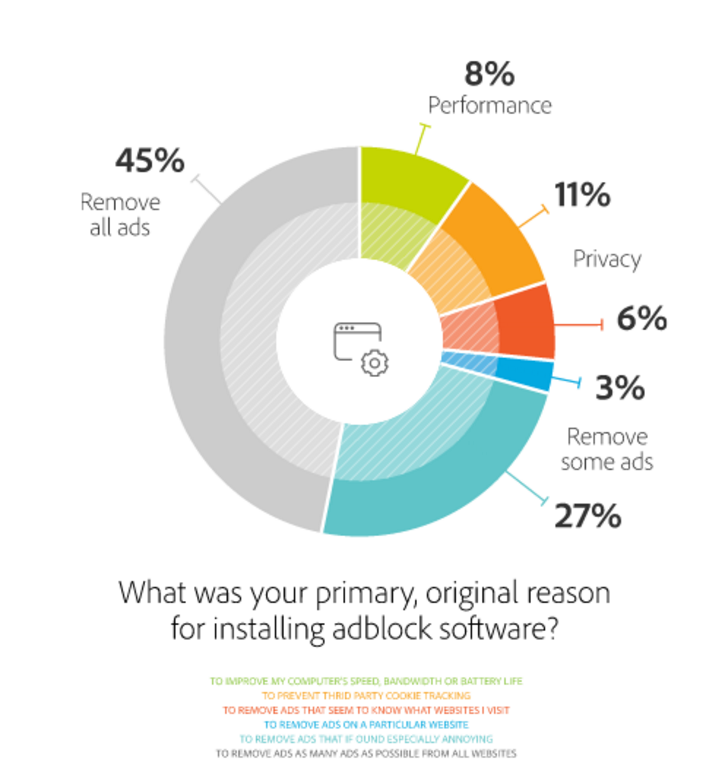
\includegraphics[width=0.75\textwidth]{whyBlockAds}
    \caption{Results of questioning why users chose to block ads \parencite{publishersWeb}}
    \label{fig:whyBlockAds}
\end{figure}

% discuss how this will effect web ecosystem (paywalls)
As technology develops and ad blocking becomes more commonplace, the growth in ad blocking usage may receive a sharp growth from mobile users,  this has the potential to challenge the viability of the web as a platform for the distribution of free ad-supported content \parencite{adobeAdBlock}. Although organisations such as Forbes have began to hide some content from users who are using ad blocking software whilst showing banners explaining they offer users a ``ad light'' version of the web page to encourage them to not use the ad blocking software, there is no guarantee that users will simply not move to the next content supplier who does not have such restrictions \parencite{publishersWeb}. Other organisations such as GQ have taken a different approach, asking users to disable their ad blocker to view their content or pay a small fee such as 50 cents per article \parencite{gq}.  This vicious cycle could see the end of the ``free web'' where information is supported via the use of adverts and in turn create an Internet littered with ``Paywalls'' where users must have a paid subscription to access content. Although Internet users may see some adverts as intrusive and annoying, the use of ad blocking software is having a detrimental effect on the web ecosystem which is so heavily reliant upon advertising. If a solution is not found, that pleases both parties, such that users are no longer faced with intrusive and annoying adverts that impede their browsing, and content providers are still able to provide their content using the funding of ads then there may be some balance. However, if a solution is not found the content and knowledge of the web could be locked behind many Paywalls which would be detrimental for all web users. \\

\section{Conclusion}
Ultimately the web ecosystem is complicated and diverse. The dependency upon advertising to fund the ``Free web'' has created an environment over-reliant on advertising to support itself. The ecosystem is over populated with ubiquitous intrusive tracking and advertising, even when privacy conscious users attempt to avoid these types of monitoring, techniques such as browser fingerprinting make it impossible for web users to avoid some form of profiling. This paper has delved into the various areas used to generate targeted advertising, attempting to bring these techniques to the forefront to expose them to users so they may be combated to return privacy to the hands of the users. \\

However, the genie is effectively out of the bottle; returning privacy to the hands of the users would require combined pressure from governments, standards organisations and web users which is unlikely to happen. An alternative model to the ``Free web'' in terms of advertising would be ``paywalls'' were information on web pages is only displayed to paying customers, which would create a fractured ecosystem where only users with enough money would be able to access the vast amount of information available on the Internet which is an outcome that would be detrimental for society as a whole. \\

In comparison to the wealth of information and free content available on the web, targeted advertising is a small price to pay. Personally, I feel that users would feel much more comfortable with the process if it was made more transparent by organisations explaining how their tracking procedure is conducted and allowing users to potentially opt-out. To conclude, whilst the techniques used to generate targeted advertising are insidious, the majority of adverts on the web do not impede web usage, these adverts underpin the majority of the free content on the web so are ultimately beneficial for almost all users of the Internet.

\medskip
\printbibliography

\end{document}
